\documentclass[11pt,a4paper]{article}

\usepackage[margin=1in]{geometry}
\usepackage{amsmath,amssymb,amsthm}
\usepackage{booktabs}
\usepackage{array}
\usepackage{listings}
\usepackage{xcolor}
\usepackage[expansion=false]{microtype}
\usepackage{enumitem}
\usepackage{tikz}
\usepackage{float}
\usepackage{algorithm}
\usepackage{algpseudocode}
\usepackage[hidelinks]{hyperref}

\usetikzlibrary{arrows.meta,calc,positioning,shapes.misc}

\definecolor{codebg}{HTML}{F5F5F5}
\definecolor{ribL}{HTML}{7F77DD}
\definecolor{ribR}{HTML}{1D9E75}
\definecolor{amb}{HTML}{EF9F27}
\definecolor{bad}{HTML}{D0453A}
\definecolor{oct1}{HTML}{E4E2F7}
\definecolor{oct2}{HTML}{C9C5EF}
\definecolor{oct3}{HTML}{ADA7E6}

\lstset{
  basicstyle=\ttfamily\footnotesize,
  backgroundcolor=\color{codebg},
  frame=single, framesep=4pt, rulecolor=\color{black!20},
  breaklines=true, columns=fullflexible, keepspaces=true,
  showstringspaces=false, xleftmargin=0pt, aboveskip=1em, belowskip=1em
}

\newcommand{\MUST}{\textsc{must}}
\newcommand{\MUSTNOT}{\textsc{must not}}
\newcommand{\SHOULD}{\textsc{should}}
\newcommand{\SHOULDNOT}{\textsc{should not}}
\newcommand{\MAY}{\textsc{may}}
\newcommand{\Dec}{\mathsf{Dec}}
\newcommand{\frc}{\operatorname{frac}}

\theoremstyle{definition}
\newtheorem{definition}{Definition}
\theoremstyle{plain}
\newtheorem{proposition}{Proposition}
\theoremstyle{remark}
\newtheorem*{remark}{Remark}

\title{\textbf{F1R3Skein: Drawn Distributions}\\[0.3em]
\large Weighted state machines for the pitch and duration streams\\[0.2em]
\normalsize Feature design, revision 2 --- companion to the instrument specification, revision 4}
\author{F1R3FLY.io}
\date{19 September 2026}

\begin{document}
\maketitle

\begin{abstract}
\noindent
In the instrument as built, each ribbon is the base-$b$ digit expansion of a transcendental
constant. The pitch ribbon runs in base $3d+1$ --- three octaves of a $d$-degree scale plus a rest
--- and the duration ribbon in base~5. The distribution of notes is therefore whatever the constant
happens to supply. This feature lets the musician, M, \emph{draw} that distribution instead: a
weighted state machine over the ribbon's states, one disc per state arranged in a circle, arrows
dragged from disc to disc, each arrow carrying a weight.

The design rests on one decision:
\begin{quote}
\textbf{M supplies the distribution; the constant still supplies the chance.}
\end{quote}
The digits of the constant are used as an exact, lazily-read uniform variate that drives the
machine, by interval refinement over the machine's cumulative weights. Everything the platform
already depends on survives unchanged: realisation is deterministic, performances replay exactly,
tunes remain terms, $\mathsf{Snip}(k,i_L,i_R,n)$ still addresses them, and breeding still operates
on map-agnostic material. The original instrument is recovered exactly as one machine among many
(Proposition~\ref{prop:embedding}). The editor itself is an all-or-nothing modal window: M commits
a valid machine or cancels, with no intermediate save.

Revision 2 records the decisions taken on revision 1 (\S\ref{sec:decisions}): every
recommendation is accepted, the duration vocabulary is fixed as whole note to sixteenth with index 0
the longest, and the evolution of machines is assigned to a later phase.
\end{abstract}

\tableofcontents

% =====================================================================
\section{What was reviewed}

The design is written against the \texttt{v2} branch of \texttt{F1R3FLY-io/F1R3Games}, head
\texttt{18a675a} (15 September 2026), which is where the current implementation lives:

\begin{itemize}[leftmargin=*,itemsep=2pt]
\item \texttt{design/f1r3skein-instrument-spec-v4.tex} --- the specification this feature extends,
  in particular \S3.3 (note mapping), \S7 (snip semantics and the envelope), \S8 (the performance
  trace) and \S9 (the wire protocol).
\item \texttt{design/Skein.module} --- the Theory of skeins.
\item \texttt{F1R3Skein/V2/f1r3skein/} --- the implementation: \texttt{skein-spigot} (digit
  streams, memoised, bases $2..64$), \texttt{skein-core} (\texttt{term.rs}, \texttt{envelope.rs},
  \texttt{state.rs}), \texttt{skein-proto} (protocol v4), \texttt{skein-engine}, and the visionOS
  client under \texttt{swift/SkeinClient} (\texttt{ControlPanel}, \texttt{SoundPanel},
  \texttt{Scale}, \texttt{SkeinModel}).
\end{itemize}

Four facts from the code shape everything below.
\begin{enumerate}[leftmargin=*,itemsep=2pt]
\item \textbf{Roles hold bases; only constants move.} \texttt{Skein::Weave} carries the pitch
  constant, the duration constant, the pitch base ($16$, $22$ or $37$) and the duration base (always
  \texttt{DURATION\_BASE}~$=5$). A twist exchanges the constants and nothing else.
\item \textbf{The top pitch digit is the rest.} \texttt{Envelope::render} maps digit $b-1$ of the
  pitch stream to silence (\texttt{top\_digit\_is\_rest}). It is generated silence: addressed,
  captured and bred like any note.
\item \textbf{Material is index pairs.} \texttt{realise} turns a term into \texttt{Cell}s of
  $(p,d)$ indices; the envelope alone turns indices into MIDI pitches and ticks. That is what makes
  breeding map-agnostic.
\item \textbf{Stream changes happen only while unzipped.} \texttt{Instrument::set\_streams} rejects
  with \texttt{AlreadyZipped} once a mesh exists, resets the affected cursor to zero on any change,
  and the scale picker in \texttt{SoundPanel} is disabled while zipped.
\end{enumerate}

% =====================================================================
\section{The machine}

\subsection{Definition}

Fix a role $\rho\in\{\text{pitch},\text{duration}\}$ with base $N_\rho$: $N_{\text{pitch}}=3d+1$ for
the selected scale, $N_{\text{duration}}=5$. The states are the ribbon's symbols
$D_\rho=\{0,\dots,N_\rho-1\}$, and in the pitch role state $N_\rho-1$ is the rest.

\begin{definition}[Drawn machine]
A \emph{drawn machine} for role $\rho$ is a tuple $\mathcal{M}=(N,\,E,\,w,\,\mu)$ where $N=N_\rho$,
$E\subseteq D_\rho\times D_\rho$ is the set of drawn arrows (self-loops permitted),
$w:E\to\mathbb{Q}_{>0}$ assigns each arrow a positive rational weight, and $\mu$ is the initial
distribution: either uniform over the discs of the component, or pinned to one start disc
(\S\ref{sec:start}).
\end{definition}

Write $V(E)$ for the discs incident to at least one arrow --- the discs M has actually used.
Discs outside $V(E)$ are simply never visited: drawing a machine over the diatonic discs that
ignores the top octave removes the top octave from the stream.

\subsection{Weights are relative; each row is normalised}

M's requirement is that a new arrow be labelled ``as if it were one of a cone to every other state,
all transitions equally likely and summing to one''. So the default weight of a new arrow is
\[
  w_0 \;=\; \frac{1}{N-1},
\]
$\tfrac1{21}$ for diatonic, $\tfrac1{15}$ for pentatonic, $\tfrac14$ for durations. We call this the
\emph{uniform-cone default} rather than a ``normal'' weight, to keep it clear of the Gaussian.

M will almost never draw a complete cone, so a row of drawn weights will not in general sum to one:
three default arrows out of a diatonic disc sum to $\tfrac3{21}$. Requiring M to balance every row by
hand would make the editor an arithmetic exercise. Weights are therefore \emph{relative}, and the
transition probability is the row-normalised weight
\[
  P(s\to t) \;=\; \frac{w(s,t)}{\sum_{(s,t')\in E} w(s,t')} .
\]
The editor shows both: the weight M typed on the arrow's chip, and beneath it the effective
probability. The consequence M sees is the natural one: all-default arrows out of a disc are equally
likely whatever their number, and doubling one arrow's weight makes it twice as likely as each of its
default siblings. The absolute value of $w_0$ only sets the scale against which M edits.

\subsection{Validity}
\label{sec:validity}

M must end the activity with either a valid machine or a cancellation. A machine is valid when:

\begin{description}[leftmargin=1.1cm,style=sameline,itemsep=3pt]
\item[\textbf{V1}] \emph{Non-empty.} $E\neq\varnothing$.
\item[\textbf{V2}] \emph{Every arrow weighted.} $w(e)\in\mathbb{Q}_{>0}$ for every $e\in E$. This
  holds by construction, since an arrow is born carrying $w_0$; the editor refuses zero or negative
  entries and offers deletion instead, because a zero-weight arrow and an absent arrow are the same
  machine.
\item[\textbf{V3}] \emph{One connected component.} The undirected graph on $V(E)$ is connected. This
  is M's stated rule.
\item[\textbf{V4}] \emph{No dead ends.} Every disc in $V(E)$ has at least one outgoing arrow.
\item[\textbf{V5}] \emph{Right size.} $N$ equals the current base of the role. (Relevant only at
  commit, if the scale changed while the editor was open.)
\end{description}

V4 is an addition to M's stated rule, and needs justifying. Specification~\S3.1 requires a stream
to be unbounded. A disc with arrows in but none out is a place the chain can reach and never leave,
so the ribbon would simply end there. Blocking commit and highlighting the offending discs keeps the
semantics explicit. \emph{Settled:} dead ends block commit; there is no implicit return to the
start distribution.

Two further conditions are \emph{reported but not enforced}, because they are musical choices rather
than errors. If the machine is not \emph{strongly} connected, the chain can enter a closed set of
discs and stay there; the editor shades the transient discs so M knows the opening material will not
return. That is often the intent --- an introduction that falls into an ostinato. And if the only
cycles have a common period (a strict alternation, say), the editor notes it.

% =====================================================================
\section{Realisation: the constant as dice}
\label{sec:realisation}

\subsection{Why the constant stays}

A machine alone does not determine a stream; it needs a source of chance. Three facts decide what
that source must be. Performances replay exactly from their trace (spec \S8). A tune is a term whose
realisation is a pure rewrite (spec \S7). And the research note requires a tune realised on a
player's machine to be bit-identical to the same tune realised by a validator. A seeded PRNG would
satisfy the first two; floating-point sampling would fail the third. The constant already present in
the role satisfies all three, with exact integer arithmetic --- and it keeps the instrument's
identity: the ribbon is still $\pi$, now heard through M's machine.

\subsection{Exact interval decoding}

Let the role's configuration be constant $c$ in base $b=N_\rho$, with digits $\delta_0\delta_1\dots$
of $\frc(c)$ as \texttt{skein-spigot} emits them. At driver position $q$ the unread tail denotes the
real number $x_q=\frc(b^{\,q}c)\in(0,1)$. For a row with successors $t_1<\dots<t_m$ and cumulative
probabilities $0=C_0<C_1<\dots<C_m=1$, decoding reads digits one at a time, narrowing
$x_q$ to a $b$-adic interval, until that interval lies inside a single bin $[C_{j-1},C_j)$.

\begin{algorithm}[H]
\caption{$\Dec(\text{row},q)$ --- one transition, exact}
\label{alg:dec}
\begin{algorithmic}[1]
\State $A\gets 0$;\; $k\gets 0$ \Comment{interval is $[A/b^k,\,(A+1)/b^k)$}
\Repeat
  \State $A\gets A\cdot b+\delta_{q+k}$;\; $k\gets k+1$
  \State $j\gets$ the index with $C_{j-1}\,b^k\le A$ and $(A+1)\le C_j\,b^k$, if one exists
\Until{$j$ found \textbf{or} $k=K_{\max}$}
\If{no $j$} \State $j\gets\max\{\,i : C_{i-1}b^k\le A\,\}$ \Comment{deterministic fallback}
\EndIf
\State \Return $(t_j,\;q+k)$ \Comment{next state, advanced driver position}
\end{algorithmic}
\end{algorithm}

All comparisons are integer comparisons after clearing the row's common denominator; there is no
floating point anywhere. The symbol stream of role $\rho$ is then
\[
  \sigma_0=\Dec(\mu,0)_1,\qquad (\sigma_{t+1},q_{t+1})=\Dec\big(\text{row}(\sigma_t),\,q_t\big),
\]
with $q_0$ the digits consumed drawing $\sigma_0$ (none when $\mu$ is pinned). Notch $t$ of the
ribbon displays, and meshes, $\sigma_t$.

\begin{proposition}[Termination]
For irrational $c$, the loop of Algorithm~\ref{alg:dec} terminates without the fallback.
\end{proposition}
\begin{proof}
$x_q=\frc(b^qc)$ is irrational because $c$ is, so it equals none of the rational boundaries $C_j$.
It therefore lies strictly inside its bin, at some distance $\varepsilon>0$ from both ends. After
$k$ digits the interval $[A/b^k,(A+1)/b^k)$ contains $x_q$ and has width $b^{-k}$; once
$b^{-k}<\varepsilon$ it lies inside the bin and the loop exits.
\end{proof}

All five constants are irrational, so $K_{\max}$ (proposed: 64) is a guard against pathological
inputs, not a rounding rule. It is recorded in the configuration so that it forms part of the
definition of realisation.

\subsection{The original instrument is one machine}

\begin{proposition}[Embedding]
\label{prop:embedding}
Let $\mathcal{U}_N$ be the complete machine on $N$ discs with every arrow including every self-loop
drawn at the default weight, and $\mu$ uniform. With $b=N$, the symbol stream of $\mathcal{U}_N$ is
exactly the digit stream: $\sigma_t=\delta_t$ for all $t$.
\end{proposition}
\begin{proof}
Every row normalises to $1/N$, so the bins are $[j/N,(j+1)/N)$. With $b=N$ the first digit read
places the interval $[A/N,(A+1)/N)$ exactly on bin $A$, so each draw consumes one digit and returns
it.
\end{proof}

So the feature does not replace the old design; it generalises it. Every existing tune is a tune of
$\mathcal{U}_N$, and the spigot-only code path can remain as the fast path for that case.

\subsection{Measured behaviour}

A Python prototype of Algorithm~\ref{alg:dec} (exact rationals, 6000--8000 transitions) gives:

\begin{center}
\begin{tabular}{llcc>{\raggedright\arraybackslash}p{4.3cm}}
\toprule
\textbf{Machine} & \textbf{Driver} & \textbf{digits/notch} & \textbf{max} & \textbf{observed} \\
\midrule
5 discs, mixed rows & $\pi$, base 5 & 1.38 & 6 & from disc 0 (three arrows, $\tfrac13$ each): .338 .357 .305 \\
same & $e$, base 5 & 1.35 & 6 & .325 .331 .344 \\
same & Liouville, base 5 & 1.00 & 2 & 1.000 to the first arrow, 0 to the others \\
22-disc full cone & $\pi$, base 22 & 1.96 & 5 & state frequencies .040--.051 against $\tfrac1{22}=.045$ \\
\bottomrule
\end{tabular}
\end{center}

Two things follow. Decoding is cheap: under two digits per notch on average, so realisation cost
stays within a small constant of the spigot's. And \textbf{the constant still colours the result
wherever it departs from normality.} $\pi$, $e$, $\varphi$ and $\ln 2$ are conjectured, not proved,
normal; empirically they behave as uniform dice. Liouville's constant is provably not normal --- its
digits are almost all zero --- so it drives every machine to the lowest bin of every row, turning a
drawn machine into a deterministic walk along first arrows. That is a legitimate and rather striking
instrument, but it should be a known one. \emph{Settled:} drawn machines are permitted on
Liouville's constant, and the editor \MUST{} say what it will do whenever the role's constant is
Liouville's.

\subsection{Cost and memoisation}

A drawn stream is sequential: $\sigma_t$ depends on the whole prefix. The engine keeps, per
(configuration, machine), a vector of symbols and a sparse table of checkpoints $(t,\sigma_t,q_t)$
every 256 notches, so re-realising a visited range is $O(1)$ per notch as spec \S3.1 requires, and a
first visit to depth $t$ costs $O(t)$ decoder steps over already-memoised digits. This is the
resource floor the research note wants: deep addresses cost more than shallow ones.

% =====================================================================
\section{Where the machine lives}

\subsection{In the term, not the envelope}

The envelope is \emph{interpretation}: given indices, which pitches and which ticks. The machine
decides \emph{which indices occur}. The same $\mathsf{Snip}(k,i_L,i_R,n)$ read through two machines
yields different material. The machine is therefore material, and belongs in the skein:

\begin{lstlisting}
pub enum Skein {
    Weave {
        pitch: Constant, duration: Constant,
        pitch_base: u32, duration_base: u32,
        pitch_machine: Option<Machine>,     // None: the plain spigot
        duration_machine: Option<Machine>,
    },
    Twist(Box<Skein>),
}
\end{lstlisting}

This keeps each existing law intact.
\begin{itemize}[leftmargin=*,itemsep=2pt]
\item \textbf{Twist.} Machines are sized by their role, so they stay with the role, like the bases:
  \[\mathsf{Twist}(\mathsf{Wv}\,p\,d\,p_b\,d_b\,p_m\,d_m)=\mathsf{Wv}\,d\,p\,p_b\,d_b\,p_m\,d_m .\]
  After a twist, $e$ drives the pitch machine and $\pi$ the duration machine. The involution still
  follows from the one equation.
\item \textbf{Snip.} Unchanged in form. $i_L,i_R$ index notch positions $t$, not driver digits.
\item \textbf{Material and breeding.} \texttt{realise} replaces \texttt{cache.range(cfg, i, n)} with
  \texttt{symbols(role, i, n)}; \texttt{Cell}s are still $(p,d)$ pairs. $\mathsf{XPitch}$,
  $\mathsf{XDur}$, $\mathsf{Pad}$ and the mutations operate on material and need no change, so
  crossing a tune drawn from a machine with a tune drawn from a bare spigot is already defined.
\item \textbf{Envelope.} Unchanged. The rest is still applied at render time, so a pitch machine
  that makes state $N-1$ likely is a machine that phrases with silence.
\end{itemize}

\subsection{Canonical form}

Tunes are de-duplicated by normalisation, so the machine is stored canonically: arrows sorted by
(source, target), each row normalised to reduced rationals, $\mu$ recorded as \texttt{Uniform} or
\texttt{Pinned(s)}. Two drawings that differ only by scaling a row are the same distribution and the
same term. Inline storage is right for \texttt{skein/v0}; on the shard a machine becomes a
content-addressed value referenced by digest, since one machine will head many tunes.

\subsection{Scale changes}

A pitch machine is a machine on $3d+1$ discs. Changing between maps of equal cardinality --- major,
minor, Dorian --- changes the envelope only, and the machine survives: the discs relabel and the
material is untouched. Changing cardinality (pentatonic to diatonic) invalidates it. The engine
\MUST{} then drop the pitch machine along with resetting the cursor, as \texttt{set\_streams}
already does for a base change, and the panel \MUST{} ask before doing so, naming the machine that
will be lost. Nothing is kept in reserve; there are no intermediate saves in this version.

\subsection{The Theory}

\texttt{Skein.module} gains a \texttt{Machines} theory. The arrows of a machine are unordered, so
they are a \texttt{HashBag} --- the collection sort the frozen grammar already supplies, unlike the
\texttt{List} that $\mathsf{Seq}$ still awaits.

\begin{lstlisting}
Theory Machines(k: Counting) {
  k
    Types   { Weight; Arrow; Init; Machine; }
    Exports { Machine; }
    Terms {
      Ratio  . p:Nat, q:Nat                    |- p "/" q                        : Weight;
      Arr    . s:Nat, t:Nat, w:Weight          |- s "->" t "@" w                 : Arrow;
      Unif   .                                 |- "uniform"                      : Init;
      Pin    . s:Nat                           |- "start" s                      : Init;
      Mach   . n:Nat, i:Init, es:HashBag(Arrow)
             |- "machine" n i "{" es.*sep(",") "}"                            : Machine;
    }
}
\end{lstlisting}

$\mathsf{Wv}$ then takes two \texttt{Option(Machine)} arguments and the twist equation is restated
as above. Row normalisation is a canonicalisation performed by the normaliser, not an equation, since
it is not expressible as a finite set of rewrite rules over \texttt{Nat} without division. One
pre-existing discrepancy should be fixed at the same time: the module's \texttt{Weave} still swaps
whole streams under $\mathsf{Twist}$, whereas \texttt{skein/v0} swaps constants only (\S\ref{sec:findings}).

% =====================================================================
\section{The editor}

\subsection{Entry and exit}

The \texttt{streams} section at the top of \texttt{ControlPanel} gains two buttons:
\textbf{Pitch distribution\ldots} and \textbf{Duration distribution\ldots}. Each opens a third
window, \texttt{WindowGroup(id: "machine", for: Role.self)}, alongside the panel and the sound
window; one editor at a time. Under each ribbon label the panel shows its source: ``$\pi$ base 22'' or
``$\pi$ base 22 $\cdot$ drawn (9 discs, 14 arrows)''.

The editor is modal in the sense M asked for.

\begin{figure}[H]\centering
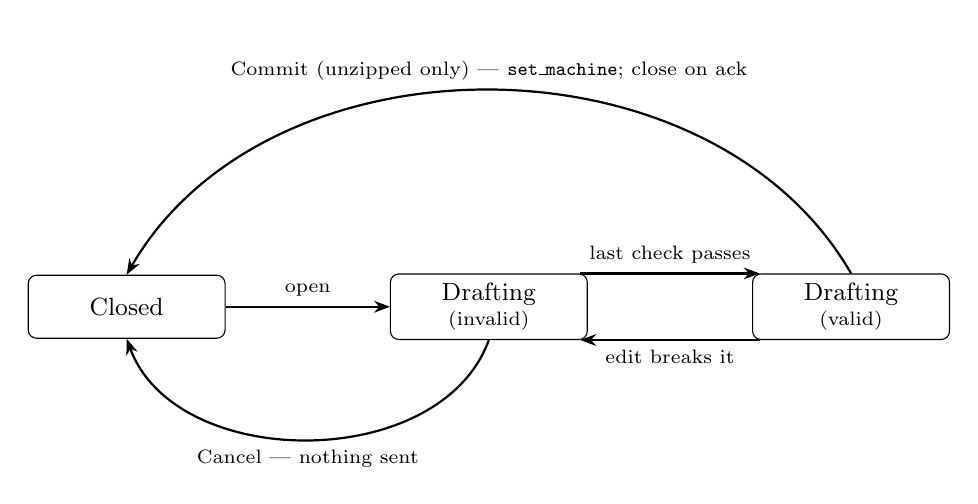
\begin{tikzpicture}[
  st/.style={draw,rounded corners=3pt,minimum width=2.5cm,minimum height=0.8cm,font=\small,align=center},
  ar/.style={-{Stealth[length=2mm]},thick}]
\node[st] (closed) at (0,0) {Closed};
\node[st] (draft) at (4.6,0) {Drafting\\[-2pt]\scriptsize(invalid)};
\node[st] (ready) at (9.2,0) {Drafting\\[-2pt]\scriptsize(valid)};
\draw[ar] (closed) -- node[above,font=\scriptsize]{open} (draft);
\draw[ar] (draft.20) -- node[above,font=\scriptsize]{last check passes} (ready.160);
\draw[ar] (ready.200) -- node[below,font=\scriptsize]{edit breaks it} (draft.340);
\draw[ar] (draft.south) to[out=-110,in=-70] node[below,font=\scriptsize]{Cancel --- nothing sent} (closed.south);
\draw[ar] (ready.north) to[out=120,in=60] node[above,font=\scriptsize]{Commit (unzipped only) --- \texttt{set\_machine}; close on ack} (closed.north);
\end{tikzpicture}
\caption{Editor lifecycle. Cancel is available in both drafting states; Commit only when valid and
unzipped.}
\end{figure}

\begin{itemize}[leftmargin=*,itemsep=2pt]
\item \textbf{Commit} is enabled only when V1--V5 hold \emph{and} the instrument is unzipped. It
  sends one \texttt{set\_machine} message; the window closes on the engine's acknowledgement and
  stays open, with the reason shown, on a rejection.
\item \textbf{Cancel} discards the draft and sends nothing. The engine never sees an unfinished
  machine, which is the whole of the ``no intermediate save points'' rule.
\item The editor \MAY{} be opened while zipped. M can draft while the wave runs; the Commit button
  says ``unzip to apply'', mirroring the scale picker.
\item Opening seeds the canvas with the role's current machine, if any, so an edit is a revision
  rather than a redraw. A \textbf{Clear} control empties the canvas, and \textbf{Use the constant}
  commits \texttt{None}, returning the role to the bare spigot.
\end{itemize}

\subsection{Layout}

\begin{figure}[H]\centering
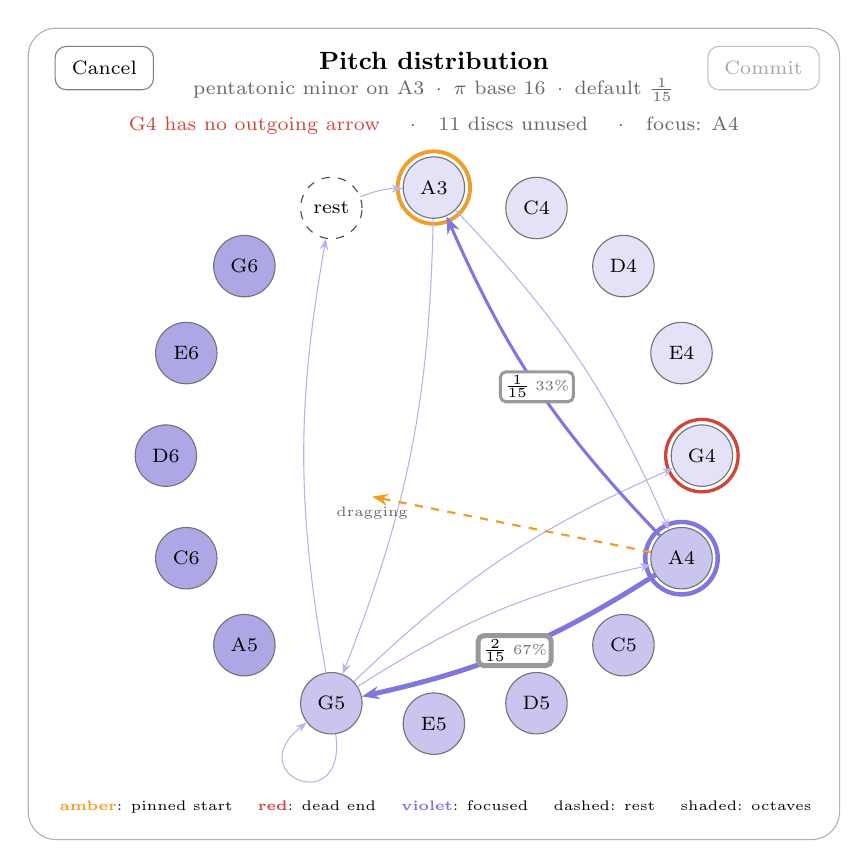
\begin{tikzpicture}[scale=0.92,
  disc/.style={circle,draw=black!55,minimum size=0.78cm,inner sep=0pt,font=\scriptsize},
  arr/.style={-{Stealth[length=2.2mm]},thick,draw=ribL},
  chip/.style={draw=black!40,fill=white,rounded corners=2pt,inner sep=1.5pt,font=\tiny},
  hair/.style={-{Stealth[length=1.4mm]},draw=ribL!55,line width=0.4pt},
  btn/.style={draw=black!50,rounded corners=4pt,minimum height=0.55cm,font=\scriptsize,inner xsep=6pt}]
% window frame
\draw[black!30,rounded corners=10pt] (-5.6,-5.3) rectangle (5.6,5.9);
% top bar
\node[btn] at (-4.55,5.35) {Cancel};
\node[font=\small\bfseries] at (0,5.45) {Pitch distribution};
\node[font=\scriptsize,black!60] at (0,5.05) {pentatonic minor on A3 \,$\cdot$\, $\pi$ base 16 \,$\cdot$\, default $\tfrac1{15}$};
\node[btn,draw=black!25,text=black!35] at (4.55,5.35) {Commit};
\node[font=\scriptsize,text=bad] at (0,4.55) {G4 has no outgoing arrow \quad\textcolor{black!60}{$\cdot$\quad 11 discs unused \quad$\cdot$\quad focus: A4}};
% discs
\def\R{3.7}
\foreach \i/\lab/\col in {0/A3/oct1,1/C4/oct1,2/D4/oct1,3/E4/oct1,4/G4/oct1,
                          5/A4/oct2,6/C5/oct2,7/D5/oct2,8/E5/oct2,9/G5/oct2,
                          10/A5/oct3,11/C6/oct3,12/D6/oct3,13/E6/oct3,14/G6/oct3}{
  \node[disc,fill=\col] (d\i) at ({90-\i*22.5}:\R) {\lab};
}
\node[disc,fill=white,dashed,draw=black!70] (d15) at ({90-15*22.5}:\R) {rest};
% start marker on A3
\draw[amb,line width=1.4pt] (d0) circle (0.5);
% bad disc G4
\draw[bad,line width=1.2pt] (d4) circle (0.5);
% focused disc
\draw[ribL,line width=1.6pt] (d5) circle (0.5);
% unfocused arrows: hairlines, thickness ~ probability, no chips
\draw[hair] (d0) to[bend left=10] (d5);
\draw[hair] (d0) to[bend left=10] (d9);
\draw[hair] (d9) to[bend left=10] (d4);
\draw[hair] (d9) to[bend left=10] (d5);
\draw[hair] (d9) to[bend left=10] (d15);
\draw[hair] (d9) to[out=-82,in=-142,looseness=7] (d9);
\draw[hair] (d15) to[bend left=10] (d0);
% focused disc's arrows, with chips
\draw[arr,line width=1.8pt] (d5) to[bend left=10] node[chip,pos=.5]{$\tfrac2{15}$\;\textcolor{black!55}{67\%}} (d9);
\draw[arr,line width=1.1pt] (d5) to[bend left=10] node[chip,pos=.5]{$\tfrac1{15}$\;\textcolor{black!55}{33\%}} (d0);
% rubber band in progress
\draw[-{Stealth[length=2mm]},dashed,amb,thick] (d5) -- ($(d5)!0.6!(d12)$) node[below,font=\tiny,text=black!60]{dragging};
% legend
\node[font=\tiny,align=left,anchor=west] at (-5.3,-4.85)
  {\textcolor{amb}{\textbf{amber}}: pinned start \quad
   \textcolor{bad}{\textbf{red}}: dead end \quad \textcolor{ribL}{\textbf{violet}}: focused \quad
   dashed: rest \quad shaded: octaves};
\end{tikzpicture}
\caption{The pitch editor for pentatonic minor: sixteen discs, fifteen pitches over three octaves
plus the rest. A4 is focused, so its two arrows carry chips showing the weight as entered and the
effective probability; every other arrow is a hairline. The draft is invalid --- G4 has arrows in but none out --- so Commit is disabled and the reason is stated
at the top, where it is legible.}
\label{fig:pitch}
\end{figure}

Discs are placed clockwise from twelve o'clock in index order, so pitch rises around the circle and
the rest sits just before the lowest note. Labels come from the envelope in force (root and map), so
the same machine relabels when M switches between equal-cardinality maps. Octaves are shaded; the
rest disc is hollow and dashed, since it is the one disc that is not a pitch.

\begin{figure}[H]\centering
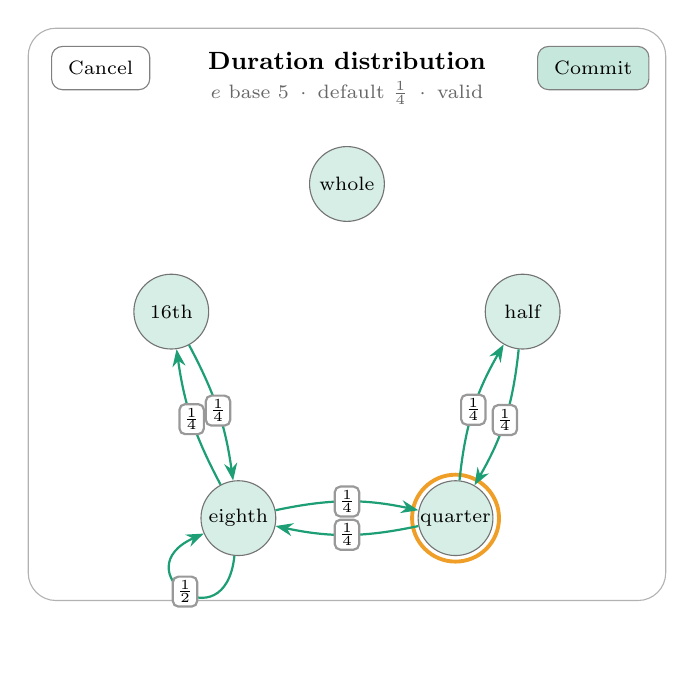
\begin{tikzpicture}[scale=0.92,
  disc/.style={circle,draw=black!55,fill=ribR!18,minimum size=0.95cm,inner sep=0pt,font=\scriptsize,align=center},
  arr/.style={-{Stealth[length=2.2mm]},thick,draw=ribR},
  chip/.style={draw=black!40,fill=white,rounded corners=2pt,inner sep=1.5pt,font=\tiny},
  btn/.style={draw=black!50,rounded corners=4pt,minimum height=0.55cm,font=\scriptsize,inner xsep=6pt}]
\draw[black!30,rounded corners=10pt] (-4.4,-3.2) rectangle (4.4,4.7);
\node[btn] at (-3.4,4.15) {Cancel};
\node[font=\small\bfseries] at (0,4.25) {Duration distribution};
\node[btn,fill=ribR!25] at (3.4,4.15) {Commit};
\node[font=\scriptsize,black!60] at (0,3.8) {$e$ base 5 \,$\cdot$\, default $\tfrac14$ \,$\cdot$\, valid};
\def\R{2.55}
\foreach \i/\lab in {0/whole,1/half,2/quarter,3/eighth,4/16th}{
  \node[disc] (d\i) at ({90-\i*72}:\R) {\lab};
}
\draw[amb,line width=1.4pt] (d2) circle (0.6);
\draw[arr] (d2) to[bend left=12] node[chip]{$\tfrac14$} (d3);
\draw[arr] (d3) to[bend left=12] node[chip]{$\tfrac14$} (d2);
\draw[arr] (d3) to[out=90-3*72+30,in=90-3*72-30,looseness=6] node[chip]{$\tfrac12$} (d3);
\draw[arr] (d3) to[bend left=10] node[chip]{$\tfrac14$} (d4);
\draw[arr] (d4) to[bend left=10] node[chip]{$\tfrac14$} (d3);
\draw[arr] (d2) to[bend left=12] node[chip]{$\tfrac14$} (d1);
\draw[arr] (d1) to[bend left=12] node[chip]{$\tfrac14$} (d2);
\end{tikzpicture}
\caption{The duration editor: five discs. This machine lives mostly on quarters and eighths, lingers
on eighths (the self-loop at $\tfrac12$ against two $\tfrac14$ siblings gives probability
$\tfrac12$), and never plays a whole note. Valid, so Commit is live.}
\label{fig:dur}
\end{figure}

\subsection{Interactions}

\begin{description}[leftmargin=1cm,style=nextline,itemsep=3pt]
\item[Draw an arrow] Look at a source disc and pinch; move the pinched hand. A rubber-band arrow
  follows the hand's projected position on the window plane. Releasing over a disc (snap radius one
  disc diameter) creates the arrow with weight $w_0$; releasing over empty space creates nothing.
\item[Self-loop] Drag out beyond the disc and back onto it. A minimum excursion distinguishes this
  from an accidental pinch-and-release, which only focuses the disc.
\item[Duplicate] Drawing an arrow that already exists does not create a second one; it opens the
  existing arrow's weight editor. $E$ is a set.
\item[Edit a weight] Tap the arrow's chip. A popover offers a fraction or decimal field (\texttt{2/15},
  \texttt{0.25}), steppers $\times2$ and $\div2$, \textbf{Reset to $w_0$}, and \textbf{Delete arrow}.
  Entry is converted to a reduced rational immediately; zero and negative entries are refused with
  the suggestion to delete. The popover also shows the whole row's resulting probabilities, since
  changing one weight changes its siblings' share.
\item[Focus] Tapping a disc focuses it: its outgoing arrows and their chips come forward, every other
  arrow fades to a hairline whose thickness still encodes probability. With 22 or 37 discs a full
  drawing can hold hundreds of arrows, and chips for all of them cannot be legible at once.
\item[Start disc] See \S\ref{sec:start}. A long pinch on a disc pins it as the start (amber ring);
  the same on the pinned disc unpins it.
\item[Undo] Within the draft only. Undo is not a save point; it disappears with the window.
\end{description}

\subsection{Validation feedback}

After every edit the editor asks the engine to check the draft (\S\ref{sec:protocol}) and paints the
answer: dead ends ringed in red, discs outside the main component dimmed, transient discs hatched,
and the first blocking problem stated in words in the header. When the machine is valid the header
shows the \emph{stationary distribution} as a thin bar inside each disc, so M sees which notes the
machine will favour over a long run --- the most useful single fact about a drawn distribution, and
one that is not obvious from the weights.

\subsection{Ergonomics on the headset}

The sound window already moved its dismiss control to the top because gaze tracking is least
reliable low in a window, and the September testing found the panel's footer buttons hard to
select. The editor follows that lesson: Cancel and Commit sit in the top bar, as do the validation
messages. Discs are at least 60\,pt, the visionOS minimum target; for chromatic, 37 discs of 60\,pt
with spacing need a ring of radius about 450\,pt, so the window's default size is 1000\,$\times$\,1000\,pt
and the ring scales down with it. Chips are also 60\,pt targets, which is a second reason chips are
shown only for the focused disc.

\subsection{The start disc}
\label{sec:start}

The initial distribution $\mu$ defaults to uniform over $V(E)$; the first symbol is then drawn from
the constant like every other. That default is what makes Proposition~\ref{prop:embedding} exact.
M may instead pin a start disc --- to begin on the tonic, say --- in which case no digits are consumed
for $\sigma_0$. Pinning is optional and never a validity condition.

% =====================================================================
\section{Engine and protocol}
\label{sec:protocol}

\subsection{Core}

\begin{lstlisting}
// skein-core/src/machine.rs
pub struct Ratio { pub num: u32, pub den: u32 }          // reduced, > 0
pub struct Arrow { pub from: u8, pub to: u8, pub weight: Ratio }
pub enum   Init  { Uniform, Pinned(u8) }
pub struct Machine { pub states: u32, pub init: Init, pub arrows: Vec<Arrow> } // canonical

impl Machine {
    pub fn canonical(self) -> Machine;                     // sort, normalise rows, reduce
    pub fn check(&self, base: u32) -> Report;               // V1..V5 + warnings + stationary
}
pub struct ChainStream { /* cfg, machine, symbols, checkpoints */ }
impl ChainStream { pub fn range(&mut self, cache: &mut DigitCache, from: usize, n: usize) -> Vec<u8>; }
\end{lstlisting}

Validation lives in \texttt{skein-core}, for the reason the implementation README gives for putting
the gesture detectors there: one implementation, unit-testable, shared by configurations S1 and S2.
The client does not re-implement V1--V5.

\subsection{Messages (protocol v5)}

\begin{center}
\begin{tabular}{l>{\raggedright\arraybackslash}p{5.2cm}>{\raggedright\arraybackslash}p{5.2cm}}
\toprule
\textbf{Type} & \textbf{Fields} & \textbf{Note} \\
\midrule
\multicolumn{3}{l}{\emph{client $\to$ engine}}\\
\texttt{check\_machine} & \texttt{role}, \texttt{machine}, \texttt{seq} &
  side-effect free; debounced to 10\,Hz while M edits \\
\texttt{set\_machine} & \texttt{role}, \texttt{machine} or \texttt{null} &
  \texttt{null} returns the role to the bare spigot \\
\midrule
\multicolumn{3}{l}{\emph{engine $\to$ client}}\\
\texttt{machine\_report} & \texttt{role}, \texttt{seq}, \texttt{valid}, \texttt{problems},
  \texttt{warnings}, \texttt{stationary} & answers a check; stale \texttt{seq} ignored \\
\texttt{machine\_ack} & \texttt{role}, \texttt{digest} & commit accepted; cursor reset to 0 \\
\texttt{rejected} & \texttt{reason}: \texttt{already\_zipped} $|$ \texttt{machine\_invalid} & existing message, new reason \\
\texttt{state} & $+$\,\texttt{pitch\_source}, \texttt{duration\_source} & labels and digests \\
\bottomrule
\end{tabular}
\end{center}

\texttt{digits} is unchanged in shape; its values are now notch symbols $\sigma_t$, which coincide
with digits for a bare spigot. \texttt{set\_machine} is accepted only while unzipped, like every
stream change, and resets the role's cursor to zero because the same position now names a different
sequence.

\subsection{Trace}

Every accepted \texttt{set\_machine} is a trace record carrying the canonical machine, and the
opening declaration of a trace includes both roles' sources. Without these the trace cannot replay a
session, which spec \S8 requires. Checks are not recorded; nothing M did in an editor she cancelled
reaches the trace.

% =====================================================================
\section{Findings from the review}
\label{sec:findings}

Three pre-existing issues touch this feature and should be resolved with it.

\begin{enumerate}[leftmargin=*,itemsep=3pt]
\item \textbf{\texttt{setScale} resets the pitch constant to $\pi$.} \texttt{SkeinModel.setScale}
  sends \texttt{configure} with \texttt{pitchConstant: "pi"} hard-coded. After a twist the pitch
  role holds $e$; changing scale then silently puts $\pi$ back and zeroes the cursor. With machines
  this matters more, because a scale change will also be the event that drops a pitch machine. The
  panel should send the constant the engine reports, or omit it.
\item \textbf{The Theory and the code disagree about twist.} \texttt{Skein.module} states
  $(\mathsf{Twist}\,(\mathsf{Wv}\,l\,r))=(\mathsf{Wv}\,r\,l)$ over whole streams; \texttt{term.rs}
  swaps constants and keeps role bases. The code is the settled design (``roles hold the bases; only
  the constants move''), and the machine extension depends on it, so the module should be brought
  into line.
\item \textbf{The musical duration map is not the one intended.} \texttt{DurationMap::Musical} is
  thirty-second, sixteenth, eighth, quarter, half, in that index order. \emph{Settled:} the musical
  vocabulary is whole note to sixteenth, with index 0 the longest:
  \begin{center}
  \begin{tabular}{lccccc}
  \toprule
  index & 0 & 1 & 2 & 3 & 4 \\
  value & whole & half & quarter & eighth & sixteenth \\
  ticks (480 per quarter) & 1920 & 960 & 480 & 240 & 120 \\
  \bottomrule
  \end{tabular}
  \end{center}
  \texttt{Musical} is changed in place rather than joined by a new map, so the four maps the
  specification requires (\S3.3) are unchanged in name. Because a trace records the map by name, a
  trace written under protocol v4 would replay with the new values; the engine therefore keeps the
  old table as a legacy entry selected by the trace's protocol version, so v4 traces still replay
  exactly. Disc labels in the duration editor are taken from this table.

  One consequence to note, not a decision: \texttt{Exponential} ($60\cdot2^i$) still runs from
  shortest to longest. If ``index 0 is the longest'' is meant to hold for every duration map, it
  should be reversed in the same change.

  Separately, the specification's base range (2--36) trails the code (2--64), which base 37 for
  chromatic needs; specification revision 5 should adopt the code's range.
\end{enumerate}

% =====================================================================
\section{Conformance}

\begin{enumerate}[leftmargin=*,itemsep=2pt]
\item $\mathcal{U}_N$ with uniform $\mu$ realises to the digit stream, for $N\in\{5,16,22,37\}$ and
  every constant (Proposition~\ref{prop:embedding}).
\item A capture taken under a drawn machine re-realises to what was heard.
\item Realisation is bit-identical across runs, processes and configurations S1 and S2.
\item $\mathsf{Twist}$ swaps constants and leaves both machines with their roles; twist is an
  involution.
\item Canonical form: row-proportional drawings are equal terms; arrow order does not matter.
\item \texttt{check} rejects each of: empty, disconnected, dead end, non-positive weight, wrong size;
  and accepts a non-strongly-connected machine with a warning.
\item \texttt{set\_machine} is rejected while zipped and resets the cursor when accepted.
\item A same-cardinality map change keeps the pitch machine; a cardinality change drops it.
\item Cancel produces no message other than checks, and no trace record.
\item Statistical (not a proof): over $10^5$ transitions driven by $\pi$, $e$, $\varphi$ and
  $\ln2$, observed transition frequencies fall within a $\chi^2$ tolerance of the machine's.
  Liouville is characterised separately: it always takes the first arrow of each row.
\item Decoder termination: no call reaches $K_{\max}$ over the test corpus.
\item \texttt{Musical} maps indices $0..4$ to $1920,960,480,240,120$ ticks, and a v4 trace replays
  under the legacy table to what was heard.
\end{enumerate}

% =====================================================================
\section{Plan of work}

\begin{description}[leftmargin=1cm,style=nextline,itemsep=3pt]
\item[\textbf{D1 --- Core.}] \texttt{machine.rs}: types, canonicalisation, \texttt{check},
  Algorithm~\ref{alg:dec}, \texttt{ChainStream} with checkpoints; extend \texttt{Skein::Weave};
  route \texttt{realise} and \texttt{Instrument::ribbon} through symbols; the new \texttt{Musical}
  table with its legacy entry (finding~3). Conformance items 1--6, 10--12. Fully testable without a
  headset.
\item[\textbf{D2 --- Engine and protocol.}] v5 messages, cursor reset, scale-change rule, trace
  records. Items 7--9. Fix finding~1.
\item[\textbf{D3 --- Editor.}] The \texttt{machine} window, discs, drag, chips, focus, popover,
  validation paint, stationary bars. Brought up in the Simulator with pointer input first, as the
  panel was.
\item[\textbf{D4 --- On device.}] Pinch-drag accuracy, snap radius and self-loop excursion tuned on
  the Vision Pro; the 37-disc chromatic ring is the stress case.
\item[\textbf{D5 --- Theory.}] \texttt{Machines} in \texttt{Skein.module}; twist equation brought
  into line (finding~2). Independent of D2--D4.
\end{description}

% =====================================================================
\section{Decisions settled}
\label{sec:decisions}

Revision 1 asked for eight decisions. All recommendations were accepted; the duration vocabulary was
fixed; and the evolution of machines was deferred.

\begin{center}
\begin{tabular}{>{\raggedright\arraybackslash}p{3.1cm}>{\raggedright\arraybackslash}p{9.6cm}}
\toprule
\textbf{Question} & \textbf{Decision} \\
\midrule
Dead ends & Block commit (V4). No implicit return to $\mu$. \\
Start & $\mu$ uniform over $V(E)$ by default; M may pin a start disc (\S\ref{sec:start}). \\
Self-loops & Permitted. The uniform cone counts every \emph{other} state, so $w_0=1/(N-1)$. \\
Duration vocabulary & Whole note to sixteenth; index 0 is the longest. \texttt{Musical} changed in
  place, with a legacy table for v4 traces (\S\ref{sec:findings}, finding 3). \\
Seeding & The editor opens on the role's current machine; \textbf{Clear} starts blank. \\
Driver & Exact lazy decoding, Algorithm~\ref{alg:dec}. \\
Liouville & Permitted, with a notice in the editor that it walks first arrows. \\
Machines as breeding material & Out of scope for this feature; a later phase. \\
\bottomrule
\end{tabular}
\end{center}

\subsection*{Deferred: evolving distributions}

Machines are terms, so they can be bred as tunes are --- crossover taking rows from each parent,
mutation perturbing weights --- letting the population evolve distributions as well as melodies.
Nothing in this design forecloses that: machines are canonical, content-addressable, and carried in
the skein. It is recorded here so that the later phase starts from the representation already
chosen.

\end{document}
